% **************************************************************************************************************
% A Classic Thesis Style
% An Homage to The Elements of Typographic Style
%
% Copyright (C) 2018 André Miede and Ivo Pletikosić
%
% If you like the style then I would appreciate a postcard. My address
% can be found in the file ClassicThesis.pdf. A collection of the
% postcards I received so far is available online at
% http://postcards.miede.de
%
% License:
% This program is free software; you can redistribute it and/or modify
% it under the terms of the GNU General Public License as published by
% the Free Software Foundation; either version 2 of the License, or
% (at your option) any later version.
%
% This program is distributed in the hope that it will be useful,
% but WITHOUT ANY WARRANTY; without even the implied warranty of
% MERCHANTABILITY or FITNESS FOR A PARTICULAR PURPOSE.  See the
% GNU General Public License for more details.
%
% You should have received a copy of the GNU General Public License
% along with this program; see the file COPYING.  If not, write to
% the Free Software Foundation, Inc., 59 Temple Place - Suite 330,
% Boston, MA 02111-1307, USA.
%
% PLEASE SEE ALSO THE AUTHORS' NOTE REGARDING THIS LICENSE
% IN THE DOCUMENTATION (ClassicThesis.pdf --> Chapter 1 / Chapter01.tex)
% **************************************************************************************************************
\RequirePackage{silence} % :-\
    \WarningFilter{scrreprt}{Usage of package `titlesec'}
    \WarningFilter{scrreprt}{Usage of package `tocloft'}
    %\WarningFilter{scrreprt}{Activating an ugly workaround}
    \WarningFilter{titlesec}{Non standard sectioning command}
\documentclass[ twoside,openright,titlepage,numbers=noenddot,%1headlines,
                headinclude,footinclude,cleardoublepage=empty,abstract=on,
                BCOR=5mm,paper=a4,fontsize=11pt, parskip
                ]{scrreprt}

%********************************************************************
% Note: Make all your adjustments in here
%*******************************************************
% LTex: enabled=false
% ****************************************************************************************************
% classicthesis-config.tex
% formerly known as loadpackages.sty, classicthesis-ldpkg.sty, and classicthesis-preamble.sty
% Use it at the beginning of your ClassicThesis.tex, or as a LaTeX Preamble
% in your ClassicThesis.{tex,lyx} with \input{classicthesis-config}
% ****************************************************************************************************
% If you like the classicthesis, then I would appreciate a postcard.
% My address can be found in the file ClassicThesis.pdf. A collection
% of the postcards I received so far is available online at
% http://postcards.miede.de
% ****************************************************************************************************


% ****************************************************************************************************
% 0. Set the encoding of your files. UTF-8 is the only sensible encoding nowadays. If you can't read
% äöüßáéçèê∂åëæƒÏ€ then change the encoding setting in your editor, not the line below. If your editor
% does not support utf8 use another editor!
% ****************************************************************************************************
\PassOptionsToPackage{utf8}{inputenc}
\usepackage{inputenc}

\PassOptionsToPackage{T1}{fontenc} % T2A for cyrillics
\usepackage{fontenc}


% ****************************************************************************************************
% 1. Configure classicthesis for your needs here, e.g., remove "drafting" below
% in order to deactivate the time-stamp on the pages
% (see ClassicThesis.pdf for more information):
% ****************************************************************************************************
\PassOptionsToPackage{
  drafting=false,    % print version information on the bottom of the pages
  tocaligned=false, % the left column of the toc will be aligned (no indentation)
  dottedtoc=true,  % page numbers in ToC flushed right
  eulerchapternumbers=true, % use AMS Euler for chapter font (otherwise Palatino)
  linedheaders=false,       % chaper headers will have line above and beneath
  floatperchapter=true,     % numbering per chapter for all floats (i.e., Figure 1.1)
  eulermath=false,  % use awesome Euler fonts for mathematical formulae (only with pdfLaTeX)
  beramono=true,    % toggle a nice monospaced font (w/ bold)
  palatino=true,    % deactivate standard font for loading another one, see the last section at the end of this file for suggestions
  style=classicthesis % classicthesis, arsclassica
}{classicthesis}


% ****************************************************************************************************
% 2. Personal data and user ad-hoc commands (insert your own data here)
% ****************************************************************************************************
\newcommand{\myTitle}{Improving Primary Key Detection\linebreak[1] with Machine Learning\xspace}
\newcommand{\myTitleHyperref}{Improving Primary Key Detection with Machine Learning\xspace}
\newcommand{\mySubtitle}{\xspace}
\newcommand{\myDegree}{Bachelor Thesis\xspace}
\newcommand{\myName}{Janek Prange\xspace}
\newcommand{\myProf}{Prof. Dr. Ziawasch Abedjan\xspace}
\newcommand{\myOtherProf}{Prof. Dr. Sören Auer\xspace}
\newcommand{\mySupervisor}{Prof. Dr. Ziawasch Abedjan\xspace}
\newcommand{\myFaculty}{Fakultät für Elektrotechnik und Informatik\xspace}
\newcommand{\myDepartment}{Institut für Praktische Informatik\xspace}
\newcommand{\myUni}{Leibniz Universität Hannover\xspace}
\newcommand{\myLocation}{Hannover\xspace}
\newcommand{\myTime}{03.07.2022\xspace}
\newcommand{\myVersion}{\classicthesis}

% ********************************************************************
% Setup, finetuning, and useful commands
% ********************************************************************
\providecommand{\mLyX}{L\kern-.1667em\lower.25em\hbox{Y}\kern-.125emX\@}
\newcommand{\ie}{i.\,e.}
\newcommand{\Ie}{I.\,e.}
\newcommand{\eg}{e.\,g.}
\newcommand{\Eg}{E.\,g.}
% ****************************************************************************************************


% ****************************************************************************************************
% 3. Loading some handy packages
% ****************************************************************************************************
% ********************************************************************
% Packages with options that might require adjustments
% ********************************************************************
\PassOptionsToPackage{ngerman, american}{babel} % change this to your language(s), main language last
% Spanish languages need extra options in order to work with this template
%\PassOptionsToPackage{spanish,es-lcroman}{babel}
\usepackage{babel}

\usepackage{csquotes}
\PassOptionsToPackage{%
  %backend=biber,bibencoding=utf8, %instead of bibtex
  backend=bibtex8,bibencoding=ascii,%
  language=auto,%
  % style=numeric-comp,%
  %style=authoryear-comp, % Author 1999, 2010
  %bibstyle=authoryear,dashed=false, % dashed: substitute rep. author with ---
  sorting=nyt, % name, year, title
  maxbibnames=10, % default: 3, et al.
  %backref=true,%
  natbib=true % natbib compatibility mode (\citep and \citet still work)
}{biblatex}
\usepackage{biblatex}
\DeclareFieldFormat{url}{\newline\mkbibacro{URL}\addcolon\nobreakspace\url{#1}}

\PassOptionsToPackage{fleqn}{amsmath}       % math environments and more by the AMS
\usepackage{amsmath}

\usepackage[strict]{changepage} %Veränderungen an Textblöcken
\usepackage{bm}

% ********************************************************************
% General useful packages
% ********************************************************************
\usepackage{graphicx} %
\usepackage{scrhack} % fix warnings when using KOMA with listings package
\usepackage{xspace} % to get the spacing after macros right
\PassOptionsToPackage{printonlyused,smaller}{acronym}
\usepackage{acronym} % nice macros for handling all acronyms in the thesis
%\renewcommand{\bflabel}[1]{{#1}\hfill} % fix the list of acronyms --> no longer working
%\renewcommand*{\acsfont}[1]{\textsc{#1}}
%\renewcommand*{\aclabelfont}[1]{\acsfont{#1}}
%\def\bflabel#1{{#1\hfill}}
\def\bflabel#1{{\acsfont{#1}\hfill}}
\def\aclabelfont#1{\acsfont{#1}}
% ****************************************************************************************************
%\usepackage{pgfplots} % External TikZ/PGF support (thanks to Andreas Nautsch)
%\usetikzlibrary{external}
%\tikzexternalize[mode=list and make, prefix=ext-tikz/]
% ****************************************************************************************************


% ****************************************************************************************************
% 4. Setup floats: tables, (sub)figures, and captions
% ****************************************************************************************************
\usepackage{tabularx} % better tables
\setlength{\extrarowheight}{3pt} % increase table row height
\newcommand{\tableheadline}[1]{\multicolumn{1}{l}{\spacedlowsmallcaps{#1}}}
\newcommand{\myfloatalign}{\centering} % to be used with each float for alignment
\usepackage{subfig}
% ****************************************************************************************************


% ****************************************************************************************************
% 5. Setup code listings
% ****************************************************************************************************
\usepackage{listings}
%\lstset{emph={trueIndex,root},emphstyle=\color{BlueViolet}}%\underbar} % for special keywords
\lstset{language=[LaTeX]Tex,%C++,
  morekeywords={PassOptionsToPackage,selectlanguage},
  keywordstyle=\color{RoyalBlue},%\bfseries,
  basicstyle=\small\ttfamily,
  %identifierstyle=\color{NavyBlue},
  commentstyle=\color{Green}\ttfamily,
  stringstyle=\rmfamily,
  numbers=none,%left,%
  numberstyle=\scriptsize,%\tiny
  stepnumber=5,
  numbersep=8pt,
  showstringspaces=false,
  breaklines=true,
  %frameround=ftff,
  %frame=single,
  belowcaptionskip=.75\baselineskip
  %frame=L
}
% ****************************************************************************************************


%*****************************************************************************************************
% 5.5 Theorems, Lemmas, Corollaries, and Proofs
%*****************************************************************************************************
\RequirePackage{amsmath}
\RequirePackage{amssymb}
\RequirePackage{theorem}
\theoremstyle{plain} {
  \newtheorem{Theorem}{Theorem}
  \newtheorem{Proposition}{Proposition}
  \newtheorem{Lemma}{Lemma}
  \newtheorem{Corollary}{Corollary}
}
\theoremstyle{plain} {\theorembodyfont{\normalfont}
  \newtheorem{Definition}{Definition}}
\newcommand{\qed}{\hfill \mbox{\raggedright \rule{.07in}{.1in}}}
\newenvironment{proof}{\vspace{1ex}\noindent{\textbf{Proof}}\hspace{0.5em}}
{\hfill\qed\vspace{2ex}}

% ****************************************************************************************************


% ****************************************************************************************************
% 6. Last calls before the bar closes
% ****************************************************************************************************
% ********************************************************************
% Her Majesty herself
% ********************************************************************
\usepackage{classicthesis}


% ********************************************************************
% Fine-tune hyperreferences (hyperref should be called last)
% ********************************************************************
\hypersetup{%
  %draft, % hyperref's draft mode, for printing see below
  colorlinks=true, linktocpage=true, pdfstartpage=3, pdfstartview=FitV,%
  % uncomment the following line if you want to have black links (e.g., for printing)
  %colorlinks=false, linktocpage=false, pdfstartpage=3, pdfstartview=FitV, pdfborder={0 0 0},%
  breaklinks=true, pageanchor=true,%
  pdfpagemode=UseNone, %
  % pdfpagemode=UseOutlines,%
  plainpages=false, bookmarksnumbered, bookmarksopen=true, bookmarksopenlevel=1,%
  hypertexnames=true, pdfhighlight=/O,%nesting=true,%frenchlinks,%
  urlcolor=CTurl, linkcolor=CTlink, citecolor=CTcitation, %pagecolor=RoyalBlue,%
  %urlcolor=Black, linkcolor=Black, citecolor=Black, %pagecolor=Black,%
  pdftitle={\myTitleHyperref},%
  pdfauthor={\textcopyright\ \myName, \myUni, \myFaculty},%
  pdfsubject={},%
  pdfkeywords={},%
  pdfcreator={pdfLaTeX},%
  pdfproducer={LaTeX with hyperref and classicthesis}%
}


% ********************************************************************
% Setup autoreferences (hyperref and babel)
% ********************************************************************
% There are some issues regarding autorefnames
% http://www.tex.ac.uk/cgi-bin/texfaq2html?label=latexwords
% you have to redefine the macros for the
% language you use, e.g., american, ngerman
% (as chosen when loading babel/AtBeginDocument)
% ********************************************************************
\makeatletter
\@ifpackageloaded{babel}%
{%
  \addto\extrasamerican{%
    \renewcommand*{\figureautorefname}{Figure}%
    \renewcommand*{\tableautorefname}{Table}%
    \renewcommand*{\partautorefname}{Part}%
    \renewcommand*{\chapterautorefname}{Chapter}%
    \renewcommand*{\sectionautorefname}{Section}%
    \renewcommand*{\subsectionautorefname}{Section}%
    \renewcommand*{\subsubsectionautorefname}{Section}%
  }%
  \addto\extrasngerman{%
    \renewcommand*{\paragraphautorefname}{Absatz}%
    \renewcommand*{\subparagraphautorefname}{Unterabsatz}%
    \renewcommand*{\footnoteautorefname}{Fu\"snote}%
    \renewcommand*{\FancyVerbLineautorefname}{Zeile}%
    \renewcommand*{\theoremautorefname}{Theorem}%
    \renewcommand*{\appendixautorefname}{Anhang}%
    \renewcommand*{\equationautorefname}{Gleichung}%
    \renewcommand*{\itemautorefname}{Punkt}%
  }%
  % Fix to getting autorefs for subfigures right (thanks to Belinda Vogt for changing the definition)
  \providecommand{\subfigureautorefname}{\figureautorefname}%
}{\relax}
\makeatother


% ********************************************************************
% Development Stuff
% ********************************************************************
\listfiles
%\PassOptionsToPackage{l2tabu,orthodox,abort}{nag}
%  \usepackage{nag}
%\PassOptionsToPackage{warning, all}{onlyamsmath}
%  \usepackage{onlyamsmath}


% ****************************************************************************************************
% 7. Further adjustments (experimental)
% ****************************************************************************************************
% ********************************************************************
% Changing the text area
% ********************************************************************
%\areaset[current]{312pt}{761pt} % 686 (factor 2.2) + 33 head + 42 head \the\footskip
%\setlength{\marginparwidth}{7em}%
%\setlength{\marginparsep}{2em}%

% ********************************************************************
% Using different fonts
% ********************************************************************
%\usepackage[oldstylenums]{kpfonts} % oldstyle notextcomp
% \usepackage[osf]{libertine}
%\usepackage[light,condensed,math]{iwona}
%\renewcommand{\sfdefault}{iwona}
%\usepackage{lmodern} % <-- no osf support :-(
%\usepackage{cfr-lm} %
%\usepackage[urw-garamond]{mathdesign} <-- no osf support :-(
%\usepackage[default,osfigures]{opensans} % scale=0.95
%\usepackage[sfdefault]{FiraSans}
% \usepackage[opticals,mathlf]{MinionPro} % onlytext
% ********************************************************************
%\usepackage[largesc,osf]{newpxtext}
%\linespread{1.05} % a bit more for Palatino
% Used to fix these:
% https://bitbucket.org/amiede/classicthesis/issues/139/italics-in-pallatino-capitals-chapter
% https://bitbucket.org/amiede/classicthesis/issues/45/problema-testatine-su-classicthesis-style
% ********************************************************************
% ****************************************************************************************************
\usepackage{pgfplots} % External TikZ/PGF support (thanks to Andreas Nautsch)
\pgfplotsset{compat=newest}
\pgfplotsset{plot coordinates/math parser=false}

%********************************************************************
% Bibliographies
%*******************************************************
\addbibresource{literatur.bib}

%********************************************************************
% Hyphenation
%*******************************************************
%\hyphenation{put special hyphenation here}

% ********************************************************************
% GO!GO!GO! MOVE IT!
%*******************************************************
\begin{document}
\frenchspacing{}
\raggedbottom{}
% \selectlanguage{ngerman} % american ngerman
%\renewcommand*{\bibname}{new name}
%\setbibpreamble{}
\pagenumbering{roman}
\pagestyle{plain}
%********************************************************************
% Frontmatter
%*******************************************************
\pdfbookmark[0]{Preamble}{preamble}
% %*******************************************************
% Little Dirty Titlepage
%*******************************************************
\thispagestyle{empty}
%\pdfbookmark[1]{Titel}{title}
%*******************************************************
\begin{center}
    \spacedlowsmallcaps{\myName} \\ \medskip

    \begingroup
        \color{CTtitle}\spacedallcaps{\myTitle}
    \endgroup
\end{center}

%*******************************************************
% Titlepage
%*******************************************************
%%%
%%% title page (german)
%%%
\pdfbookmark[1]{Titlepage}{title}
\begin{titlepage}
  \changetext{}{21mm}{}{19mm}{}
  \vspace{1cm}
  \begin{center}
    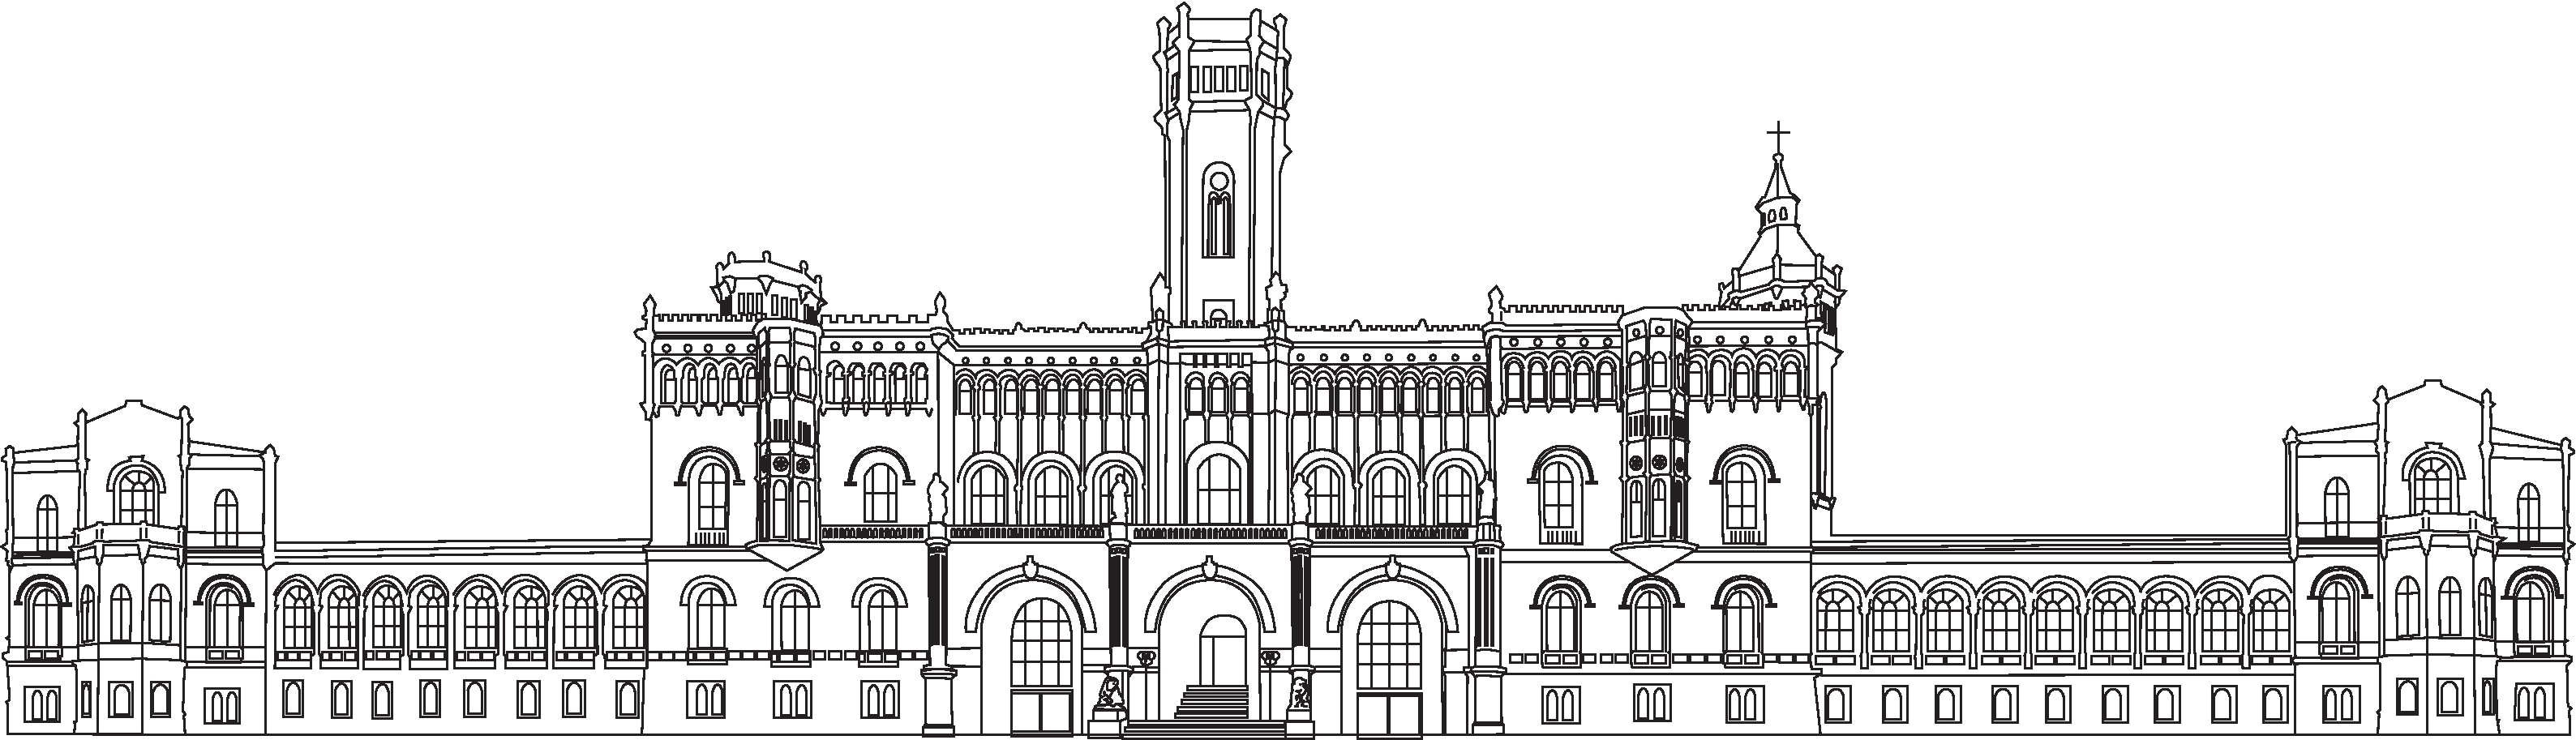
\includegraphics[width=13.8cm]{img/welfenschloss} \\
  \end{center}
  \medskip
  \begin{center}
    \textbf{\huge\spacedallcaps{L}\LARGE\spacedallcaps{eibniz}}
    \textbf{\huge\spacedallcaps{U}\LARGE\spacedallcaps{niversit\"{a}t}}
    \textbf{\huge\spacedallcaps{H}\LARGE\spacedallcaps{annover}} \\
  \end{center}

  \begin{center}
    \normalsize
    \spacedallcaps{Fakult\"{a}t}
    \spacedallcaps{f\"{u}r}
    \spacedallcaps{Elektrotechnik}
    \spacedallcaps{und}
    \spacedallcaps{Informatik} \\
    \smallskip
    \spacedallcaps{Institut}
    \spacedallcaps{f\"{u}r}
    \spacedallcaps{Praktische Informatik}
  \end{center}
  \vfill
  \vfill


  {
    %*******************************************************
    % Titlepage for everyone else 
    %*******************************************************
    \begin{center}
      \LARGE \myTitle{}
    \end{center}
    \vfill
    \vfill

    \begin{center}
      \LARGE \textbf{\myDegree}
    \end{center}
    \vfill

    \begin{center}
      \large submitted by \\
    \end{center}

    \begin{center}
      \large \spacedallcaps{\myName}
    \end{center}

    \begin{center}
      \large on \myTime{} \\
    \end{center}
    \vfill

    \begin{center}
      \begin{tabular}{lll}
        First Examiner  & : & \myProf{}       \\ % chktex 26
        Second Examiner & : & \myOtherProf{}  \\ % chktex 26
        Supervisor      & : & \mySupervisor{} % chktex 26
      \end{tabular}
    \end{center}

  }  % end condWIWI

  %  \vfill

  %  \begin{center}
  %    \large \selectedthesisnumber \\
  %  \end{center}

  \changetext{}{-21mm}{}{-19mm}{}

\end{titlepage}

\thispagestyle{empty}

\hfill

\vfill

\noindent\myName: \textit{\myTitle,}
%\mySubtitle,
%\myDegree,
\textcopyright{}~\myTime{}

%\bigskip
%
%\noindent\spacedlowsmallcaps{Supervisors}: \\
%\myProf \\
%\myOtherProf \\
%\mySupervisor
%
%\medskip
%
%\noindent\spacedlowsmallcaps{Location}: \\
%\myLocation
%
%\medskip
%
%\noindent\spacedlowsmallcaps{Time Frame}: \\
%\myTime

\cleardoublepage{}
%*******************************************************
% Declaration
%*******************************************************
\pdfbookmark[1]{Declaration}{declaration}
\chapter*{Declaration}
\thispagestyle{empty}
I hereby affirm that I have completed this work without the help of third parties and only with the sources and aids indicated. All passages that were taken from the sources, either verbatim or in terms of content, have been marked as such. This work has not yet been submitted to any examination authority in the same or a similar form.
\bigskip

\noindent\textit{\myLocation{}, \myTime{}}

\smallskip

\begin{flushright}
    \begin{tabular}{m{5cm}}
        \\ \hline % chktex 44
        \centering\myName{} \\
    \end{tabular}
\end{flushright}

% \cleardoublepage{}
% %*******************************************************
% Dedication
%*******************************************************
\thispagestyle{empty}
\phantomsection{}
\pdfbookmark[1]{Dedication}{Dedication}

\vspace*{3cm}

\begin{center}
    \emph{Ohana} means family. \\
    Family means nobody gets left behind, or forgotten. \\ \medskip
    --- Lilo \& Stitch
\end{center}

\medskip

\begin{center}
    Dedicated to the loving memory of Rudolf Miede. \\ \smallskip
    1939\,--\,2005
\end{center}

\cleardoublepage{}
%*******************************************************
% Abstract
%*******************************************************
%\renewcommand{\abstractname}{Abstract}
\pdfbookmark[1]{Abstract}{Abstract}
% \addcontentsline{toc}{chapter}{\tocEntry{Abstract}}
\begingroup
\let\clearpage\relax
\let\cleardoublepage\relax
\let\cleardoublepage\relax
%! TODO
\chapter*{Abstract}
The discovery of primary key candidates and unique columns in general is an important problem. % TODO: write better
The current algorithms to find unique columns are not fast enough for large tables as their runtime depends on the size of the table.

In this thesis, I propose a new method to detect unique columns. It uses a machine learning model to predict which columns are probably unique columns. Only positive guesses will be checked for duplicates. With this method, the time it takes to detect all unique columns is reduced by more than \SI{60}{\percent} for large tables with more than \num{10000000} rows. % TODO: is this number correct?

\endgroup


\cleardoublepage{}
% LTex: enabled=false
%*******************************************************
% Table of Contents
%*******************************************************
\pagestyle{scrheadings}
%\phantomsection
\pdfbookmark[1]{\contentsname}{tableofcontents}
\setcounter{tocdepth}{2} % <-- 2 includes up to subsections in the ToC
\setcounter{secnumdepth}{3} % <-- 3 numbers up to subsubsections
\manualmark{}
\markboth{\spacedlowsmallcaps{\contentsname}}{\spacedlowsmallcaps{\contentsname}}
\tableofcontents{}
\automark[section]{chapter}
\renewcommand{\chaptermark}[1]{\markboth{\spacedlowsmallcaps{#1}}{\spacedlowsmallcaps{#1}}}
\renewcommand{\sectionmark}[1]{\markright{\textsc{\thesection}\enspace\spacedlowsmallcaps{#1}}}
%*******************************************************
% List of Figures and of the Tables
%*******************************************************
\clearpage
% \pagestyle{empty} % Uncomment this line if your lists should not have any headlines with section name and page number
\begingroup
\let\clearpage\relax
\let\cleardoublepage\relax
%*******************************************************
% List of Figures
%*******************************************************
%\phantomsection
%\addcontentsline{toc}{chapter}{\listfigurename}
\pdfbookmark[1]{\listfigurename}{lof}
\listoffigures

\vspace{8ex}

%*******************************************************
% List of Tables
%*******************************************************
%\phantomsection
%\addcontentsline{toc}{chapter}{\listtablename}
\pdfbookmark[1]{\listtablename}{lot}
\listoftables

\vspace{8ex}
% \newpage

%*******************************************************
% List of Listings
%*******************************************************
%\phantomsection
%\addcontentsline{toc}{chapter}{\lstlistlistingname}
\pdfbookmark[1]{\lstlistlistingname}{lol}
\lstlistoflistings{}

\vspace{8ex}

%*******************************************************
% Acronyms
%*******************************************************
%\phantomsection
% \pdfbookmark[1]{Acronyms}{acronyms}
% \markboth{\spacedlowsmallcaps{Acronyms}}{\spacedlowsmallcaps{Acronyms}}
% \chapter*{Acronyms}
% \begin{acronym}[UMLX]
%     \acro{ai}[AI]{Artificial Intelligence}
%     \acro{auto-ml}[Auto-ML]{automated machine learning}
%     % \acro{acronym}[short name]{long name}
% \end{acronym}

\endgroup

%********************************************************************
% Mainmatter
%*******************************************************
\cleardoublepage{}
\pagestyle{scrheadings}
\pagenumbering{arabic}
% use \cleardoublepage here to avoid problems with pdfbookmark
\cleardoublepage{}

% \ctparttext{You can put some informational part preamble text here.
%     Illo principalmente su nos. Non message \emph{occidental} angloromanic
%     da. Debitas effortio simplificate sia se, auxiliar summarios da que,
%     se avantiate publicationes via. Pan in terra summarios, capital
%     interlingua se que. Al via multo esser specimen, campo responder que
%     da. Le usate medical addresses pro, europa origine sanctificate nos se.}
% \cleardoublepage{}

\chapter{Motivation}
Tables are a way to store and organize data that continues to grow in importance. Be it SQL databases, No-SQL databases or simple Excel tables, the ability to organize data and present it concisely is at the core of many projects.

In the best case, the structure of the dataset has already been considered before creating it in order to define which data type can occur in each column, whether values can be left empty and which columns act as primary keys.

However, there are cases where this information is not available for various reasons; either because the data had to be saved quickly and there was no capacity for reasonable planning, or because the data is no longer available in the original format. % TODO: maybe a citation?

In this case, it is an important task to recover the missing metadata as accurately as possible. While information such as the data type and the existence of empty values is comparatively easy to find within a linear runtime, identifying primary keys is more difficult.

One challenge is to distinguish between primary key candidates, which are characterized by the fact that they do not contain duplicates, and practically usable primary keys. An example for this is a column containing comments from users. Even though this column may not contain duplicates, text that is on average 100 characters long is not practically suitable as a key.

Another problem is the time it takes conventional algorithms to determine if a column contains duplicates. The at best linear runtime of these algorithms becomes a problem as the tables become very large and contain several million rows.

The focus of this thesis is to improve the efficiency to detect unique columns, especially for large tables.

\chapter{Problem Statement}\label{chap:problem_statement} % TODO: writing
% TODO: better first sentence
Primary key candidates are columns in a table which do not have any duplicate values and are therefore suited to identify a row in the table. In this thesis, a column that contains only distinct values, one of which is a None/Null value, is considered non-unique as it can not be used as a primary key.  % chktex 18

Runtime of naive algorithm (sorting and hashing based)

No problem with small tables, but problem with tables with more than a few million rows

% TODO: integrate into this section
The naive algorithm that is used for the experiments in Chapter~\ref{chap:experiments} is a sorting based method. However, it has the specialty of aborting if one of the values is None/Null since the column can not be used as a primary key.

The reason the hashing based method was not used for the experiments was to be able to reliably carry out the efficiency experiments. Although the sorting based method is less efficient, it enables the experiments to be set up in a way that enables the machine learning model to make the correct prediction without decreasing the runtime of the naive algorithm.

\chapter{Fundamental Knowledge}
\section{Metrics}\label{sec:metrics}
% https://towardsdatascience.com/accuracy-precision-recall-or-f1-331fb37c5cb9
During the training and testing of a machine learning model, its performance is measured with different metrics which indicate how closely the prediction of the machine learning model matches reality. Table~\ref{table:true-false-neg-pos} shows the different possible relations between prediction and reality.

\begin{table}[ht]
  \centering
  \caption{Definition of true and false negatives and positives}
  \begin{tabular}{ll|l|l} % chktex 44
                            & \multicolumn{1}{c}{} & \multicolumn{2}{c}{Prediction}                  \\
                            &                      & Negative                       & Positive       \\ \cline{2-4}
    \multirow{2}{*}{Actual} & Negative             & True Negative                  & False Positive \\ \cline{2-4}
                            & Positive             & False Negative                 & True Positive  \\
  \end{tabular}\label{table:true-false-neg-pos}
\end{table}

Four metrics exist based on those measurements to calculate the correctness of the machine learning model.

The first of these metrics is accuracy, which is calculated by dividing the number of correct guesses by the total number of guesses. It indicates how close the prediction is to the actual result and is therefore a good general reference point for the correctness of the model.

The second metric, precision, is defined as the number of true positive guesses divided by the total number of positive guesses. It is very well suited for determining the correctness when false positives are associated with a high cost.

Recall is the third metric and defined as the number of positive guesses divided by the number of actual positives. It is a good metric to measure the performance when false negatives are associated with a high cost.

Finally, F1 is calculated by dividing the product of precision and recall by their sum. Just like accuracy, F1 is well suited when both precision and recall are equally important. The difference is that F1 is especially good in cases where the number of positives and negatives is very unbalanced. An example for this is a dataset where \SI{99}{\percent} of the actual results are negatives.

\section{Machine Learning}\label{sec:machine_learning}
Machine learning is a part of the field of \ac{ai}. The focus is on extracting information from large amounts of data, with algorithms gradually improving themselves to mimic human learning~\cite{what-is-ml}.

The field of machine learning is itself divided into two main parts, Classical learning and Deep learning\cite{ml-visual-explanation}.

% https://ischoolonline.berkeley.edu/blog/what-is-machine-learning/
% https://www.ibm.com/cloud/learn/machine-learning

\subsection{Deep Learning and Neural Networks} % TODO: need to proof read

Deep Learning includes various techniques that use neural networks. In the simplest form, neural networks consist of different so-called nodes, which are arranged as layers\cite{neuralNet}.

The first layer, also known as the \enquote{input layer}, is the layer the input vector is applied to. If the input exceeds a certain value, the neuron is activated, i.e.\ it passes on an output.

In the next layers, which are called \enquote{hidden layers}, the outputs from all the nodes of the previous layer and a \enquote{bias layer} are computed in each node and the output is passed on. The bias layer consists of a single value that influences all nodes on a layer.

Finally, the last layer outputs the result of the computation. How strong each previous node influences the value of the current node is what the neural network is trained on.

Neural networks are particularly good at recognizing patterns in large unordered data, such as images, videos, and audio tracks. Examples of this include facial recognition or verifying hand signatures\cite{neuralNet-applications}.

\newcommand{\neuralx}[2]{\(x_#2\)}
\newcommand{\neuraly}[2]{\(\hat{y}_#2\)}
\newcommand{\neuralh}[2]{\small \(h^{(#1)}_#2\)}
\begin{figure}[ht]
  \centering
  \caption[An example of a neural network]{A simple neural network with three input nodes and two output nodes.}
  \begin{neuralnetwork}[height=5]
    \inputlayer[count=3, bias=false, title=Input\\layer, text=\neuralx]
    \hiddenlayer[count=4, bias=true, title=Hidden\\layer 1, text=\neuralh] \linklayers{}
    \hiddenlayer[count=3, bias=false, title=Hidden\\layer 2, text=\neuralh] \linklayers{}
    \outputlayer[count=2, title=Output\\layer, text=\neuraly] \linklayers{}
  \end{neuralnetwork}\label{fig:neural_network}
\end{figure}

\subsection{Classical Learning} % TODO: writing
% https://towardsdatascience.com/deep-learning-vs-classical-machine-learning-9a42c6d48aa
Algorithms in the field of classical machine learning are largely based on statistical or probabilistic methods, which originated as pattern recognition in the 1960s. It has the advantage of being a fast method that does not require much computing power compared to deep learning algorithms\cite{classical-ml}.

%! TODO: another paragraph

\subsection{Categories of Machine Learning}
Both deep learning as well as classical learning are dived into different categories which are based on the kind of task and trainingsdata the machine learning models have to work with.

Unsupervised learning is used on unlabeled data. Its main use is to organize the data or to make it more manageable. Tasks in this domain include clustering, which categorizes data based on similar data points, or assoziation, which tries to find relationships between variables in a dataset\cite{supervised-unsupervised-learning}.

Supervised learning on the other hand makes use of labeled data. This comes with the disadvantage that the structure of the data as well as the desired results have to be known\cite{classical-ml}. Even though it increases the effort of the preparation of the trainingsdata, it also raises the accuracy of the model since it is trained to produce exactly the desired result.

% TODO: what and why labeled data?

% Reinforcement Learning  \cite{types-of-ml} %! TODO

\begin{figure}[ht]
  \caption[Different kinds of machine learning]{This picture shows the different types of machine learning and the way they are trained\cite{types-of-ml}.} % TODO: is a more detailed description necessary?
  \centering
  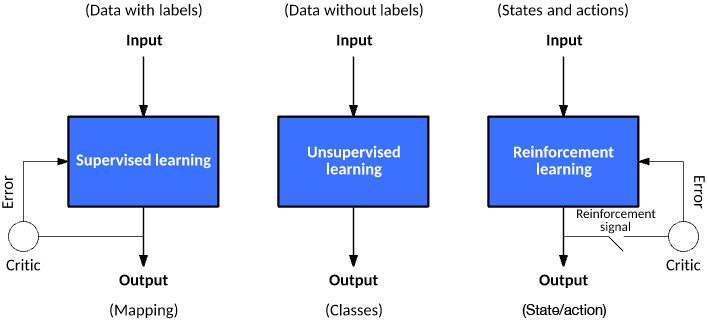
\includegraphics[width=\linewidth]{img/types_of_machine_learning.png}\label{fig:kinds_of_ml}
\end{figure}

\section{Naive Algorithms}
Here or in a subsection of Proposed Method?
\section{Used packages and libraries}\label{sec:used_packages_and_libraries} % TODO: writing

\subsection{Pandas}

\subsection{Scikit-Learn and Auto-Sklearn}

\chapter{Proposed Method}\label{chap:proposed_method}
\section{Overview}\label{sec:overview}
In this thesis I present a method to increase the efficiency of finding unique columns in a table. The method is based on a machine learning model which uses the first few rows of each column to guess if it will have any duplicate values. Each positive guess will subsequently be validated using a conventional naive method.

The proposed method works in three steps. First, the features are extracted from the first rows of the table. After that, the model tries to predict the existence of duplicate values from the features. Finally, the columns which are unique according to the model are checked with a naive method.

The source code of the proposed method as well as the experiments in Chapter~\ref{chap:experiments} can be found in the GitHub repository \url{https://github.com/LUH-DBS/Prange}.

% ["Duplicates", "Data Type", "Sorted",
%           # number
%           "Min. value", "Max. value", "Mean", "Std. Deviation",
%           # string
%           "Avg. string length", "Min. string length", "Max. string length"
%           ]  # 10
\section{Feature Extraction}\label{sec:extracted_features}
The machine learning model which is used by the proposed method can not work on the tables directly as it is trained with supervised learning. The model therefore uses a feature table as input, an example of which can be seen in Table~\ref{table:feature_table_example}.

% \begin{sidewaystable}
\begin{table}[ht]
  \caption[An example feature table]{An example for a feature table which is used by the model proposed in Chapter~\ref{chap:proposed_method}. The following values are possible in the column \enquote{Data Type}:
    \begin{enumerate*}[start=0, label={\num{\arabic*}:}]
      \item The inspected rows contain a duplicate value.
      \item The column contains only integer.
      \item The column contains only text.
      \item The column contains only boolean values (which does rarely occur without containing duplicates).
      \item The column contains a mix of different types.
    \end{enumerate*}}
  \setlength{\tabcolsep}{4pt}
  \small
  \makebox[\linewidth]{%
    \begin{tabular}{SSSSSSSSSS}
      \toprule
      {\shortstack{Duplicates}} & {\shortstack{Data                                                                                               \\Type}} & {\shortstack{Sorted}} & {\shortstack{Min.\\value}} & {\shortstack{Max.\\value}} & {\shortstack{Mean}} & {\shortstack{Std.\\Deviation}} & {\shortstack{Avg.\\string\\length}} & {\shortstack{Min.\\string\\length}} & {\shortstack{Max.\\string\\length}} \\ \midrule
      1                         & 0                 & 0 & 0.0   & 0.0   & 0.0              & 0.0              & 0.0                & 0.0  & 0.0   \\
      0                         & 1                 & 1 & 7.0   & 562.0 & 290,705882352941 & 187,488587887997 & 0.0                & 0.0  & 0.0   \\
      0                         & 1                 & 1 & 1.0   & 62.0  & 28,9411764705882 & 21,4955535757843 & 0.0                & 0.0  & 0.0   \\
      0                         & 1                 & 1 & 611.0 & 946.0 & 789,117647058824 & 107,903824279391 & 0.0                & 0.0  & 0.0   \\
      0                         & 1                 & 1 & 1.0   & 17.0  & 9,0              & 5,04975246918104 & 0.0                & 0.0  & 0.0   \\
      0                         & 2                 & 0 & 0.0   & 0.0   & 0.0              & 0.0              & 86.25              & 78.0 & 92.0  \\
      0                         & 2                 & 0 & 0.0   & 0.0   & 0.0              & 0.0              & 78.75              & 60.0 & 96.0  \\
      0                         & 2                 & 0 & 0.0   & 0.0   & 0.0              & 0.0              & 123.03225806451613 & 51.0 & 296.0 \\
      0                         & 2                 & 0 & 0.0   & 0.0   & 0.0              & 0.0              & 94.1304347826087   & 46.0 & 204.0 \\
      0                         & 3                 & 0 & 0.0   & 0.0   & 0.0              & 0.0              & 0.0                & 0.0  & 0.0   \\
      0                         & 4                 & 0 & 0.0   & 0.0   & 0.0              & 0.0              & 0.0                & 0.0  & 0.0   \\
      \bottomrule
    \end{tabular}\label{table:feature_table_example}
  }
\end{table}
% \end{sidewaystable}


% TODO: which data type numbers exist? -> is inside the text sufficient?

The code in Listing~\ref{lst:proposed_method-prepare_column} extracts the features from each column to produce such a feature table. The feature extraction of the proposed method works in different steps which are executed one after the other.

The variable column contains the first \textit{n} rows of the column in the table where \textit{n} is the input size of the method.

First all columns which contain duplicate values in the first rows are sorted out in line 1 and 2 by setting the feature \enquote{Duplicates} to \num{1} and all other features to \num{0}.

In line 5 to 12 the remaining columns are checked in order to determine whether they are sorted or not. During this step, it is possible that an error occurs because two values in the column can not be compared. This is mostly the case if there is an empty/None value in the column.

In the following lines, a distinction is made between the different types of values.

If the column contains only boolean values, the feature \enquote{Data Type} is set to \num{3} while all other features stay on \num{0} in line 13 to 16. Although it is very unlikely that a column contains exclusively boolean values without any duplicate values, there are tables in the GitTables dataset to which this applies.

Line 17 to 23 handle columns that contain exclusively numeric values. The \enquote{Data Type} feature is set to \num{1} in line 18 and the four features specific to numeric values are extracted in line 19 and 20. The three remaining features are set to \num{0} in line 22.

Finally, the columns that contain exclusively string or a mix of different types are handled in the remaining lines.

First, the features for numeric values are set to 0 in line 25. After that, the average of the length of every item in the column is formed together with the minimum and maximum length. At the end the \enquote{Data Type} feature is set to \num{2} in line 39.

If there is any value in the column which is not a string, a ValueError is raised in line 32, which leads to the \enquote{Data Type} feature being set to \num{4} in line 42 and the string specific features set to \num{0}.

It should be emphasized that the column header is not being extracted as a feature. While this could lead to a better performance in some cases, it is challenging to encode the various headings in a way that is understandable for the machine learning model.

\lstinputlisting[
  float,
  numbers=left,
  language=Python,
  caption={[The algorithm to extract the features from a column]This code shows how the features are extracted from a column. This process is repeated for each column; the result forms the feature table which is the input for the machine learning model. The variable \texttt{column} contains the first \textit{n} rows of the column where \textit{n} is the input size of the model.},
  label={lst:proposed_method-prepare_column}
]{table-code/proposed-method/prepare-columns.py}


\section{Used packages and libraries}\label{sec:used_packages_and_libraries} % TODO: maybe another paragraph?
For this thesis, the algorithms and experiments where implemented using Python 3.10.2. To interact with the data, the python library pandas was used as its dataframe structure has useful additional functions and has a good compatibility to the library Auto-Sklearn, which was used to train the machine learning model.


\section{Training the Model}\label{sec:traing_the_model}
The machine learning model was trained on the training dataset, which is a subset with \num{10000} tables of the GitTables dataset that is used for the correctness test in Section~\ref{sec:correctness}. Each of the tables has a minimum size of \num{100} rows and \num{3} columns. % TODO: write better, explain GitTables further?

From each table in the training dataset the features where extracted and saved as the \enquote{training\_data} table. Additionally, the data was correctly classified using the naive algorithm to form the \enquote{training\_result} table.

The Listing~\ref{lst:proposed_method-train_model} presents the training process. First, in line 5 and 6 the feature table produced from the training data and the result table where loaded as pandas dataframes.

In line 8 to 11, the training parameters where selected. The train time was changed for the different experiments in Chapter~\ref{chap:experiments}. The model was always trained with the metric recall used to measure its performance, as false negatives have the highest cost for the performance of the model. While there is a cost associated with false positives too, they do not decrease the correctness of the proposed method as each positive guess by the model is verified using a naive algorithm.

Finally, in line 12 the model is trained on the training data. Auto-Sklearn automatically chooses the best of a range of classical learning algorithms. % TODO: write better? 

\lstinputlisting[
  float=ht,
  numbers=left,
  language=Python,
  caption={[Training the model with Auto-Sklearn]This code shows how the machine learning model is trained using the python library Auto-Sklearn.}, % TODO: The data is loaded as pandas dataframes?
  label={lst:proposed_method-train_model}
]{table-code/proposed-method/train_model.py}

\chapter{Experiments}

\section{Correctness}\label{sec:correctness}
The correctness of the model is probably the most important metric to determine its usability. While a false positive is not a major problem for the correctness because each positive guess is verified (see Chapter~\ref{chap:proposed_method}), a false negative leads to a primary key candidate being ignored.

In this section, different experiments will be conducted to determine which parameters have an influence on the correctness of the prediction. Additionally, in Section~\ref{subsec:correctness_examine-false-guesses} the columns which led to false guesses by the model will be examined.


\subsection{Experiment Data}\label{subsec:correctness_experiment-data}
The experiments where performed on the GitTables dataset, which is a large corpus of relational tables extracted from CSV files in GitHub~\cite{gittables-article}. However, not the whole dataset was used but only a subset of tables split into a training and a test dataset.

The training dataset is used to train every model which was tested in the following experiments including the efficiency experiments. It is a subset of the GitTables dataset with \num{10000} tables which where selected by traversing the GitTables dataset and skipping tables which are too small.

Every table in it has to have at least \num{100} rows and \num{3} columns to ensure the feature extraction described in Section~\ref{lst:proposed_method-prepare_column} does not become the naive algorithm with extra steps. This could be a problem as searching for duplicates with the naive algorithm in the first \textit{n} rows of each column is part of the feature extraction.

The test dataset was generated the same way as the training dataset. By traversing the GitTables and skipping every table which is too small or part of the training dataset a collection of \num{5000} tables with \num{57211} columns and an average of \num{184} rows was generated. It was used for every experiment apart from the one in Section~\ref{subsec:correctness_comparing-input-size} where a dataset of \num{30000} tables with \num{307030} columns and an average of \num{277} rows was used.


\subsection{Comparing models with different input sizes}\label{subsec:correctness_comparing-input-size}
As described in Section~\ref{sec:extracted_features}, the proposed method extracts features from the first rows of a table and uses a machine learning model to predict if a column has any duplicate values based on those features. % TODO: is ref to extracted features correct?

In this experiment, I compare different models which use the first \num{5}, \num{10}, \num{20} and \num{50} rows of each column to extract features. A model with an input size larger than \num{50} rows was not feasible as the tables used for training and testing had a minimum size of \num{100} rows. With a bigger input, the feature extraction would end up performing like the naive algorithm as checking the first \textit{n} rows for duplicates with the naive algorithm is part of the feature extraction. % chktex 13 % TODO: is the last sentence too much? practically the same is said in the previous subsection


Each model was trained for \num{5} hours on the training dataset. During the experiment, the test dataset with \num{5000} tables that was described in Section~\ref{subsec:correctness_experiment-data} was used to test each model.

Table~\ref{table:correctness-comparing_input_sizes} shows the results of this experiment, which demonstrates that the input size has a large influence on the quality of the prediction. While none of the models has any false negative guesses, the number of false positive guesses decreases with an increasing input size.

%! TODO: how many positive guesses? -> guess_count.csv

This experiment shows that an increase in the input size of the model does have a great impact on the number of false positive guesses. However, since each positive guess by the model is verified using the naive algorithm, the number of false guesses has no effect on the quality of the final prediction of the proposed method. What is however effected by it is the efficiency of the method; this is explored further in Section~\ref{subsec:efficiency-changing_uniques}.

Another important finding of this experiment is that even with a small input size of only \num{5} rows, the model has not made any false negative guesses. As the negative guesses of the model are not checked, it is important for them to be correct to ensure the overall correctness of the proposed method.

\begin{table}[ht]
  \centering
  \caption[Result for Correctness: Comparing different input sizes]{The result of the correctness experiment comparing models with different input sizes. Each of the models was trained for \num{5} hours on \num{10000} tables. The test was conducted on \num{30000} tables with an average of \num{277} rows and a total of \num{307030} columns.} % TODO: ref to dataset description
  \begin{tabular}{S[table-format=2]SSSS}
    \toprule
    {Model Input Size} & {Accuracy}         & {Precision}         & {Recall} & {F1}               \\ \midrule
    5                  & 0.7038921278051005 & 0.2687803622558955  & 1.0      & 0.4236830427892235 \\
    10                 & 0.8329283783343647 & 0.39448025119814906 & 1.0      & 0.5657738800663664 \\
    20                 & 0.9096993779109533 & 0.546554797769164   & 1.0      & 0.7068030160425545 \\
    50                 & 0.9697521414845455 & 0.7825313195176209  & 1.0      & 0.8780000788198048 \\
    \bottomrule
  \end{tabular}\label{table:correctness-comparing_input_sizes}
\end{table}


\subsection{Altering the training time}\label{subsec:correctness_comparing-training-time}
The Auto-Sklearn library, which was used to train the machine learning models, automatically searches for the best learning algorithm and optimizes it as described in Section~\ref{sec:used_packages_and_libraries}. Since this process takes time to run, in theory the performance of the model increases with higher training time. % TODO: maybe write better? 

In this experiment, different models with an input size of \num{10} rows are being trained for different amounts of time on the training dataset. Subsequently, the experiment is conducted for each model on the test dataset with \num{5000} tables.

The Table~\ref{table:correctness-compare_training_time} presents the results of this experiment. With a training time of one minute the performance of the machine learning model is indeed slightly worse as there are some false negative guesses.

However, apart from the false negative guesses, the models with a training time of one and two minutes have a slightly better performance than the other models. % TODO: maybe write better?

This experiment very clearly demonstrates that the machine learning model does not need a long training time to find unique columns. Furthermore, it shows that there might be advantageous to train a model multiple times and compare them to find the best performing, since a longer training time does not translate to higher performance.

\begin{table}[ht]
  \centering
  \caption[Result for Correctness: Comparing different training times]{The result of the correctness experiment comparing models which were trained for different amounts of time on the training dataset. The experiment was conducted on the test dataset with \num{5000} tables.} % TODO: maybe a text more different from table compare-input-sizes
  %! TODO: number of false negatives
  \begin{tabular}{SSSSS}
    \toprule
    {Training Time [\si{\minute}]} & {Accuracy}         & {Precision}        & {Recall}          & {F1}               \\ \midrule
    1                              & 0.8465155302302005 & 0.3685386778170283 & 0.995714842228282 & 0.5379636937647987 \\
    2                              & 0.8468651133523274 & 0.3694854264123785 & 1.0               & 0.5395974565137421 \\
    5                              & 0.8231284193599133 & 0.3365895233724513 & 1.0               & 0.5036542894982097 \\
    10                             & 0.8231284193599133 & 0.3365895233724513 & 1.0               & 0.5036542894982097 \\
    20                             & 0.8231284193599133 & 0.3365895233724513 & 1.0               & 0.5036542894982097 \\
    40                             & 0.8231284193599133 & 0.3365895233724513 & 1.0               & 0.5036542894982097 \\
    60                             & 0.8231284193599133 & 0.3365895233724513 & 1.0               & 0.5036542894982097 \\
    120                            & 0.8231284193599133 & 0.3365895233724513 & 1.0               & 0.5036542894982097 \\
    180                            & 0.8231284193599133 & 0.3365895233724513 & 1.0               & 0.5036542894982097 \\
    300                            & 0.8231284193599133 & 0.3365895233724513 & 1.0               & 0.5036542894982097 \\
    \bottomrule
  \end{tabular}\label{table:correctness-compare_training_time}
\end{table}


\subsection{Summary}\label{subsec:correctness_conclusions} %! TODO
The experiments in this section demonstrate that the predictions made by the model have a sufficiently high accuracy. Models which have been trained for more than one minute had a recall of 1 and therefore no false negative guesses. This is a very good result as false negative guesses would lead to unique columns which are ignored.

Furthermore, the models in the experiments produce less than twice as much false positive guesses as true positive guesses and even less for models with a larger input size. This is important as false positive guesses reduce the efficiency, which is explored further in Section~\ref{sec:efficiency}.


\subsection{Examine columns which led to false guesses}\label{subsec:correctness_examine-false-guesses} % TODO: maybe a table with examples?
The greatest weakness of the proposed method are false guesses. False positive guesses lead to a reduced efficiency because more columns need to be checked with the naive algorithm. False negative guesses on the other hand result in primary key candidates being ignored which reduces the correctness. It is therefore important to examine the columns which lead to false guesses to improve the model if possible.

False positive guesses occur very often as the model is primarily trained to avoid any false negative guesses. The experiment in Section~\ref{subsec:correctness_comparing-input-size} has shown that depending on the input size between \SI{27}{\percent} and \SI{78}{\percent} of the positive guesses are false positives.

The false guesses are unfortunately mostly unavoidable as they are caused mainly by empty cells which are located after the input rows of the model in otherwise unique columns. As the column would be a primary key candidate without these missing values, there is no possible change which would improve the correctness of the model in this case.

Another example for a column leading to a false positive guess is one containing the name of authors. Since the model only sees short strings without duplicates in these columns, there is no good way for the current implementation to recognize the column as non-unique. However, it would be possible to additionally include the column heading as a feature to enable the model to learn that the column with the names of authors is more likely to contain duplicate values.

False negative guesses occurred only in one of all the correctness experiments, namely with the model which was trained for only one minute in Section~\ref{subsec:correctness_comparing-training-time}. And even then the false negatives were rare, and the corresponding columns contained only negative numbers or numbers smaller than 1. While these columns are negative, they are not suited very well as primary keys. % TODO: is this ok?

% TODO: Maybe a summarizing paragraph?


\section{Efficiency}\label{sec:efficiency}
Next to the correctness, the efficiency of the proposed method is the most important metric to determine its feasibility. % TODO: maybe a better wording?
The main question is if or from what table size the proposed method is faster than the naive method. This becomes even more interesting as each positive guess of the model has to be verified using the naive algorithm to increase the accuracy. % TODO: ref to model

The following experiments explore the efficiency of the proposed method in comparison to the naive algorithm and which parameters have the greatest influence on it. %! TODO: write better?


\subsection{Experiment Data}\label{subsec:efficiency-experiment_data}
The experiments in this section were conducted on a set of generated tables to control the size of the table as well as the number of unique and non-unique columns. A small example of such a table can be seen in Table~\ref{table:efficiency-generated_table}. % chktex 18

The generated tables each have \num{10} columns and between \num{100} and \num{100000000} columns. To ensure the correct prediction by the model, the columns where generated in a specific way.
The unique columns are evenly incrementing for the first \num{50} rows, while the first two rows of the non-unique columns contain the same value. The rest of each column contains distinct incrementing values which are mixed up to increase the time the sorting based naive algorithm takes to find unique columns. % TODO: ref to naive algorithm  % chktex 18

\begin{table}[!ht]
  {
    \newcommand{\tablevdots}{\multicolumn{1}{c}{\vdots{}}}
    \setlength{\tabcolsep}{5pt}
    \caption[A table generated for the efficiency experiment]{A table generated for the efficiency experiment. The columns 0 and 1 do not contain any duplicates, the columns 2, 3 and 4 do. To guarantee that the model guesses the unique and non-unique columns correctly, the unique columns are evenly incrementing for the first 50 rows, while the duplicate value of the non-unique columns is in the first two rows.}
    \begin{tabularx}{\linewidth}{X<{\centering}SSSSS}
      \toprule
      {Index}       & {Column \num{0}} & {Column \num{1}} & {Column \num{2}} & {Column \num{3}} & {Column \num{4}} \\ \midrule
      \num{0}       & 0                & 0                & 100              & 100              & 100              \\
      \num{1}       & 1                & 1                & 100              & 100              & 100              \\
      \num{2}       & 2                & 2                & 93               & 93               & 93               \\
      \num{3}       & 3                & 3                & 45               & 45               & 45               \\
      % 4        & 4                & 4                & 16               & 16               & 16               \\
      % 5        & 5                & 5                & 87               & 87               & 87               \\
      % 6        & 6                & 6                & 32               & 32               & 32               \\
      \tablevdots{} & \tablevdots{}    & \tablevdots{}    & \tablevdots{}    & \tablevdots{}    & \tablevdots{}    \\
      % 46       & 46               & 46               & 2                & 2                & 2                \\
      % 47       & 47               & 47               & 73               & 73               & 73               \\
      \num{48}      & 48               & 48               & 89               & 89               & 89               \\
      \num{49}      & 49               & 49               & 39               & 39               & 39               \\
      \num{50}      & 91               & 91               & 60               & 60               & 60               \\
      \num{51}      & 77               & 77               & 49               & 49               & 49               \\
      % 52       & 54               & 54               & 23               & 23               & 23               \\
      % 53       & 70               & 70               & 30               & 30               & 30               \\
      \bottomrule{}
    \end{tabularx}\label{table:efficiency-generated_table}

  }
\end{table}



\subsection{Base experiment}\label{subsec:efficiency-base_experiment}
The first experiment explores the efficiency of the proposed method compared to the naive algorithm. The generated tables that were used contained \num{3} unique and \num{7} non-unique columns.  % chktex 18

Figure~\ref{fig:efficiency-base_experiment-plot} and Table~\ref{table:efficiency_csv-70percent} show that for tables with up to \num{100000} rows, the naive algorithm takes only a fraction of a second and is therefore faster than the proposed machine learning model. However, since the model takes a roughly constant time of half a second to compute its prediction, it becomes faster as the table size surpasses one million rows.

The column \enquote{Model: Validation} in Table~\ref{table:efficiency_csv-70percent} additionally illustrates that the validation time of the proposed method is proportional to the number of positive guesses by the model. This highlights the importance of as few false positive guesses as possible, because each false positive guess unnecessarily increases the runtime through the required validation and therefore decreases the efficiency.

In conclusion, this experiment illustrates that for large tables loading the dataset and checking the columns for duplicates with the naive algorithm takes the most time. Possibilities to reduce the loading time will be explored in Section~\ref{subsec:efficiency-shorter_loading_times}. While a more efficient naive algorithm is not part of this thesis, Section~\ref{subsec:correctness_comparing-input-size} and~\ref{subsec:correctness_examine-false-guesses} deal with the question of how to decrease the number of false positive guesses.

\begin{figure}[ht]
  \caption[Compare the efficiency the proposed method and the naive algorithm]{This plot shows the total time for the naive algorithm and the proposed method to compute the unique columns as can be seen in Table~\ref{table:efficiency_csv-70percent}. The tables were saved in a CSV format.} % TODO: better caption
  \label{fig:efficiency-base_experiment-plot} % chktex 24
  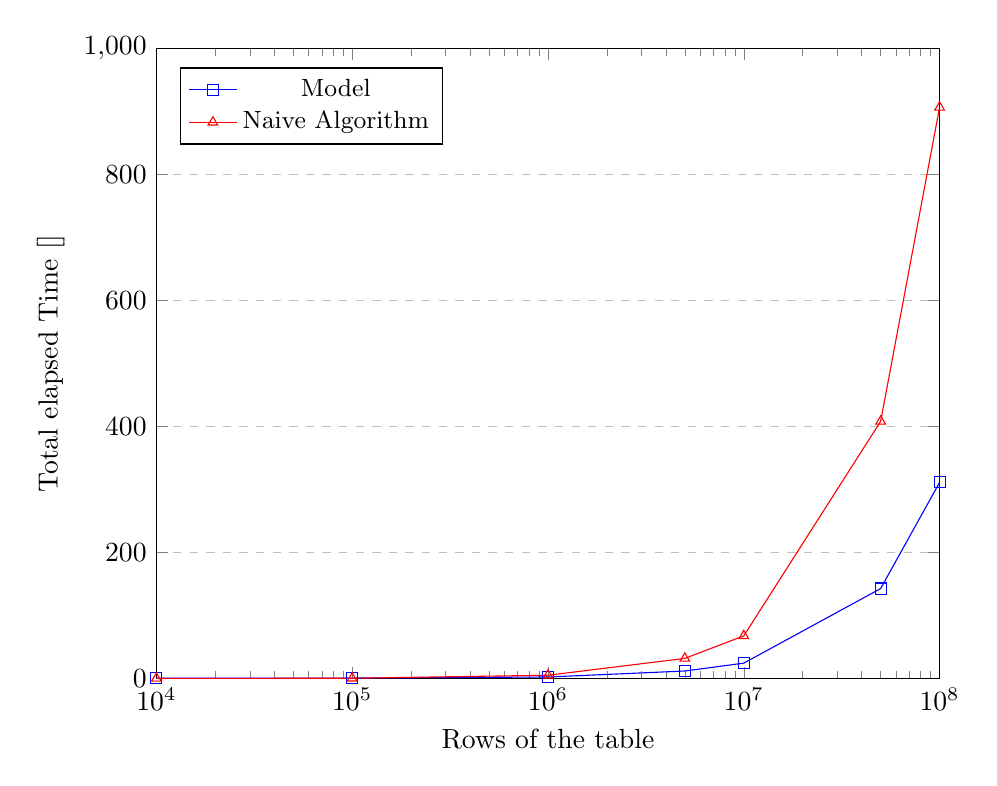
\begin{tikzpicture}
    \begin{axis}[
        % title={},
        xlabel={Rows of the table},
        ylabel={Total elapsed Time [\si{\second}]},
        xmin=10000, xmax=100000000, xmode=log,
        ymin=0, ymax=1000,
        % xtick={0,1000,100000,10000000,100000000},
        % ytick={0,20,40,60,80,100,120},
        legend pos=north west,
        ymajorgrids=true,
        grid style=dashed,
        scale only axis,
        width={\linewidth-62pt},
        height=8cm
      ]

      \addplot[
        color=blue,
        mark=square,
      ]
      coordinates {
          (100.0,1.0835406184196472) (1000.0,0.4514627978205681) (10000.0,0.4591604061424732) (100000.0,0.5741918832063675) (1000000.0,2.2600879333913326) (5000000.0,11.771335251629353) (10000000.0,24.25790297240019) (50000000.0,142.64984269440174) (100000000.0,311.1732710637152)
        };
      \addplot[
        color=red,
        mark=triangle,
      ]
      coordinates{
          (100.0,0.0039823874831199) (1000.0,0.0037141181528568) (10000.0,0.0264939442276954) (100000.0,0.3022922314703464) (1000000.0,5.0495885498821735) (5000000.0,31.796920645982027) (10000000.0,67.54112743958831) (50000000.0,408.1332451477647) (100000000.0,906.6464131213723)
        };
      \legend{\small Model, \small Naive Algorithm}

    \end{axis}
  \end{tikzpicture}
\end{figure}


\begin{table}[htb]
    \centering
    \begin{tabular}{@{}cccccccccc@{}}
        \toprule
        Rows & Columns & ML: Loading & ML: Compute Time & ML: Loading & ML: Validation Time & ML: Total & Naive: Loading & Naive: Compute Time & Naive: Total \\
        \midrule
        100 & 10 & 0.0065117068588733 & 1.901446133852005 & 0.0065117068588733 & 0.0001417063176631 & 1.90841730684042 & 0.0035603828728199 & 0.0005022697150707 & 0.0040644854307174 \\
        1000 & 10 & 0.0015828944742679 & 1.8984689489007 & 0.0015828944742679 & 0.0006108358502388 & 1.9009892046451569 & 0.0016751401126384 & 0.0019342266023159 & 0.0036102943122386 \\
        10000 & 10 & 0.0052565038204193 & 1.9095683731138704 & 0.0052565038204193 & 0.0065431855618953 & 1.921698283404112 & 0.0049404129385948 & 0.0220178365707397 & 0.0269592814147472 \\
        100000 & 10 & 0.0429374687373638 & 1.9027229472994804 & 0.0429374687373638 & 0.0742254443466663 & 2.020440120249986 & 0.0424283891916275 & 0.2558906264603138 & 0.2983216643333435 \\
        1000000 & 10 & 0.4255336932837963 & 1.903101004660129 & 0.4255336932837963 & 1.3649001717567444 & 3.696124318987131 & 0.4222380295395851 & 4.689979210495949 & 5.112221155315638 \\
        10000000 & 10 & 4.559976447373629 & 1.8975738510489464 & 4.559976447373629 & 19.02081367000937 & 25.518052734434605 & 4.547631841152906 & 63.52510995417833 & 68.0727454200387 \\
        100000000 & 10 & 51.986212998628616 & 1.90036316588521 & 51.986212998628616 & 257.835216768086 & 312.1136333048344 & 52.16438018530607 & 852.7149710021913 & 904.8793550543488 \\
        5000000 & 10 & 2.4457033053040504 & 1.8983104377985 & 2.4457033053040504 & 8.743456106632948 & 13.107568178325891 & 2.4423254802823067 & 29.05716192722321 & 31.49949196726084 \\
        50000000 & 10 & 26.75338465720415 & 1.89099595323205 & 26.75338465720415 & 114.87536582350732 & 143.71518944576383 & 27.03932445123792 & 379.5964986868202 & 406.6358272023499 \\
        \bottomrule
    \end{tabular}
\end{table}


\subsection{Reduce loading times}\label{subsec:efficiency-shorter_loading_times}
While CSV files are very easy to use, they are not meant to efficiently store large quantities of data. A file format which is substantially more suitable to handle large datasets is the parquet format~\cite{parquet-book}.

It achieves this through the use of various features such as column wise compression, which tends to be more efficient since the values in the same column are usually very similar. This has the additional benefit of enabling the algorithm to only read the required columns which may decrease \io{} as only positive guesses need to be loaded for the validation.

Another advantageous property of this format is the concept of row groups, which ensure that a batch of rows is being saved together and can therefore be read together too. This makes it possible to read just the first row group and use these rows as an input for the model.

The Table~\ref{table:efficiency_parquet-70percent} shows the result of the base experiment from Section~\ref{subsec:efficiency-base_experiment} repeated with tables generated as parquet files. While the computing time for the model and the naive algorithm remain roughly equal compared to Table~\ref{table:efficiency_csv-70percent}, the loading time is decreased significantly for large tables. %? loading times make up a larger part of total time for model

\GenericWarning{}{LaTeX Warning: This table needs to be manually checked}
\begin{table}[ht]
    \caption{The result of the efficiency test with a generated table with \SI{30}{\percent} unique columns in a parquet file format. The test was conducted on a model with an input size of 10 rows on tables with 10 columns.}
    \begin{tabular}{@{}SSSSSSSSS@{}}
        \toprule
        {\shortstack{Rows}} & {\shortstack{Model:\\Loading}} & {\shortstack{Model:\\Computing}} & {\shortstack{Model:\\Loading}} & {\shortstack{Model:\\Validation}} & {\shortstack{Model:\\Total}} & {\shortstack{Naive:\\Loading}} & {\shortstack{Naive:\\Computing}} & {\shortstack{Naive:\\Total}} \\
        \midrule
        100 & 0.0037329792976379 & 0.4535947442054748 & 0.0037329792976379 & 0.0001380555331707 & 0.4577647559344768 & 0.0056636519730091 & 0.0005674697458744 & 0.0062335357069969 \\
        1000 & 0.002842117100954 & 0.4445352330803871 & 0.002842117100954 & 0.0006063096225261 & 0.4482727721333504 & 0.0034207440912723 & 0.0018974170088768 & 0.0053194314241409 \\
        10000 & 0.003845926374197 & 0.4464297965168953 & 0.003845926374197 & 0.0065436139702796 & 0.4571339413523674 & 0.0040172487497329 & 0.0205030031502246 & 0.0245211236178874 \\
        100000 & 0.0095696412026882 & 0.4469785206019878 & 0.0095696412026882 & 0.0770864151418209 & 0.5343325138092041 & 0.0097010508179664 & 0.2462445013225078 & 0.2559473849833011 \\
        1000000 & 0.0399911925196647 & 0.462495107203722 & 0.0399911925196647 & 1.3958711363375187 & 1.90179156512022 & 0.0468120314180851 & 4.618332322686911 & 4.6651470102369785 \\
        5000000 & 0.1967337541282177 & 1.2639095708727837 & 0.1967337541282177 & 8.750608161091805 & 10.232811015099289 & 0.183550912886858 & 29.032910093665123 & 29.216464921832085 \\
        10000000 & 0.4818546883761883 & 0.4799107164144516 & 0.4818546883761883 & 18.93440898507833 & 19.938058882951736 & 0.5291252098977566 & 62.745562482625246 & 63.27469082176685 \\
        50000000 & 2.216078583151102 & 0.9870042651891708 & 2.216078583151102 & 113.88575321435928 & 117.29449190944432 & 2.2049838453531265 & 379.4684140905738 & 381.673400811851 \\
        100000000 & 4.47317860648036 & 1.5488394163548946 & 4.47317860648036 & 257.4711396209896 & 263.89783180877566 & 4.395280238240957 & 857.4373284652829 & 861.8326124921441 \\
        \bottomrule
    \end{tabular}\label{table:efficiency_parquet-70percent}
\end{table}

Table~\ref{table:efficiency_parquet-70percent_small-tables} presents the result for the experiment using the advantages of the file format by loading only the necessary rows and columns. This leads to two loading times for the model. The first time only the first row group is being loaded while the second time only the columns which are unique according to the model are loaded. However, this does not make any difference except for the largest table and even then the total time is hardly changing.

\begin{table}[ht]
    \caption[Efficiency experiment on tables with \SI{30}{\percent} unique columns saved as parquet files, where only the necessary rows and columns are loaded]{The result of the efficiency experiment conducted on a table generated with \num{3} unique and \num{7} non-unique columns saved as a parquet file. The experiment was conducted on a model with an input size of 10 rows which was trained on the training dataset. During the experiment, only the necessary rows and columns were loaded.}
    \small
    \setlength{\tabcolsep}{4pt}
    \makebox[\linewidth][r]{%
        \begin{tabular}{@{}S[table-format=9]SSSSSSSS@{}}
            \toprule
            {\shortstack{Rows}} & {\shortstack{Model:\\Loading I}} & {\shortstack{Model:\\Computing}} & {\shortstack{Model:\\Loading II}} & {\shortstack{Model:\\Validation}} & {\shortstack{Model:\\Total}} & {\shortstack{Naive:\\Loading}} & {\shortstack{Naive:\\Computing}} & {\shortstack{Naive:\\Total}} \\
            \midrule
            100                 & 0.0019583702087402  & 0.4582597687840462 & 0.0025078989565372 & 0.0001805499196052 & 0.4629099182784557 & 0.0035582929849624 & 0.0004192851483821 & 0.0039786621928215 \\
            1000                & 0.0015548579394817  & 0.4559830017387867 & 0.0025322996079921 & 0.0007521696388721 & 0.4608258455991745 & 0.0026408433914184 & 0.0018298886716365 & 0.0044715628027915 \\
            10000               & 0.0024227760732173  & 0.4511252082884311 & 0.0029931813478469 & 0.0066407360136508 & 0.4631855227053165 & 0.0039258524775505 & 0.0203023217618465 & 0.024229060858488  \\
            100000              & 0.0093600116670131  & 1.4681769870221617 & 0.006388496607542  & 0.0805302299559116 & 1.5644594952464104 & 0.0085682570934295 & 0.2470835894346237 & 0.2556539326906204 \\
            1000000             & 0.0322037003934383  & 0.454765647649765  & 0.0255185328423976 & 1.356141496449709  & 1.8686350099742413 & 0.0499729178845882 & 4.665698669850826  & 4.715674605220556  \\
            5000000             & 0.1148154400289058  & 0.4625117443501949 & 0.1057574264705181 & 8.687994543462992  & 9.371084868907928  & 0.1949679963290691 & 29.00083852931857  & 29.195809934288263 \\
            10000000            & 0.2425682730972767  & 0.4470147676765919 & 0.2583311088383198 & 18.96086385846138  & 19.90878576785326  & 0.5438475236296654 & 63.12243377417326  & 63.66628506034613  \\
            50000000            & 1.1834049336612225  & 0.447280365973711  & 1.3086804077029228 & 114.8945118971169  & 117.83388417959212 & 2.2251016534864902 & 379.7313333004713  & 381.9564390294254  \\
            100000000           & 1.6024668291211128  & 0.4462943933904171 & 2.42531206831336   & 256.9933520145714  & 261.4674338325858  & 4.437270112335682  & 856.736768040806   & 861.1740412451327  \\
            \bottomrule
        \end{tabular}\label{table:efficiency_parquet-70percent_small-tables}
    }
\end{table}

In summary, while the reduced loading time does make a notable difference, it is not very large compared to the efficiency gain achieved through the use of the proposed method, as can be seen in Figure~\ref{fig:efficiency-shorter_loading_time-plot}. This could change, however, if the file reading speed would be slower, for example because the data had to be read over the internet. In this case, reading only the necessary rows and columns and thus decreasing \io{} further could make a larger difference too.

\begin{figure}[ht]
  \caption[]{} %! TODO: better caption
  \label{fig:efficiency-shorter_loading_time-plot} % chktex 24
  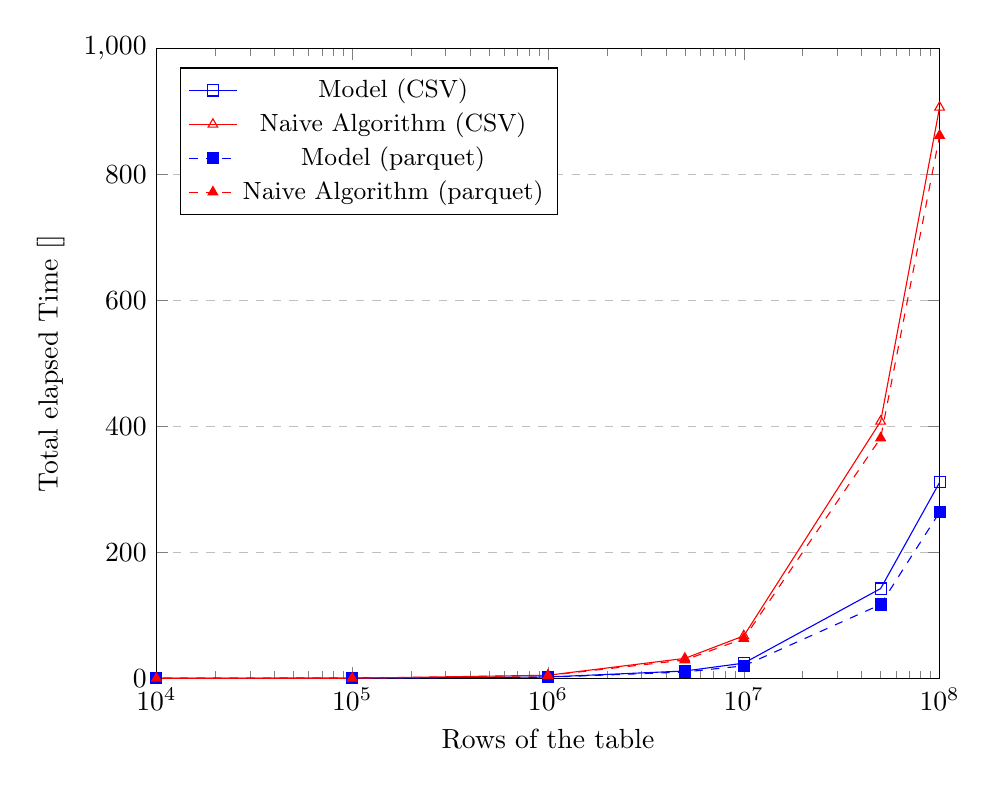
\begin{tikzpicture}
    \begin{axis}[
        % title={},
        xlabel={Rows of the table},
        ylabel={Total elapsed Time [\si{\second}]},
        xmin=10000, xmax=100000000, xmode=log,
        ymin=0, ymax=1000,
        % xtick={0,1000,100000,10000000,100000000},
        % ytick={0,20,40,60,80,100,120},
        legend pos=north west,
        ymajorgrids=true,
        grid style=dashed,
        scale only axis,
        width={\linewidth-62pt},
        height=8cm
      ]

      % csv
      \addplot[
        color=blue,
        mark=square,
      ]
      coordinates {
          (100.0,1.0835406184196472) (1000.0,0.4514627978205681) (10000.0,0.4591604061424732) (100000.0,0.5741918832063675) (1000000.0,2.2600879333913326) (5000000.0,11.771335251629353) (10000000.0,24.25790297240019) (50000000.0,142.64984269440174) (100000000.0,311.1732710637152)
        };

      \addplot[
        color=red,
        mark=triangle,
      ]
      coordinates{
          (100.0,0.0039823874831199) (1000.0,0.0037141181528568) (10000.0,0.0264939442276954) (100000.0,0.3022922314703464) (1000000.0,5.0495885498821735) (5000000.0,31.796920645982027) (10000000.0,67.54112743958831) (50000000.0,408.1332451477647) (100000000.0,906.6464131213723)
        };

      % parquet
      \addplot[
        color=blue,
        mark=square*,
        dashed,
        mark options={solid}
      ]
      coordinates {
          (100.0,0.4577647559344768) (1000.0,0.4482727721333504) (10000.0,0.4571339413523674) (100000.0,0.5343325138092041) (1000000.0,1.90179156512022) (5000000.0,10.232811015099289) (10000000.0,19.938058882951736) (50000000.0,117.29449190944432) (100000000.0,263.89783180877566)
        };

      \addplot[
        color=red,
        mark=triangle*,
        dashed,
        mark options={solid}
      ]
      coordinates{
          (100.0,0.0062335357069969) (1000.0,0.0053194314241409) (10000.0,0.0245211236178874) (100000.0,0.2559473849833011) (1000000.0,4.6651470102369785) (5000000.0,29.216464921832085) (10000000.0,63.27469082176685) (50000000.0,381.673400811851) (100000000.0,861.8326124921441)
        };

      %       % parquet small_table
      %       \addplot[
      %         color=blue,
      %         mark=square,
      %       ]
      %       coordinates {
      % (100.0,0.4629099182784557) (1000.0,0.4608258455991745) (10000.0,0.4631855227053165) (100000.0,1.5644594952464104) (1000000.0,1.8686350099742413) (5000000.0,9.371084868907928) (10000000.0,19.90878576785326) (50000000.0,117.83388417959212) (100000000.0,261.4674338325858) 
      % };

      %       \addplot[
      %         color=red,
      %         mark=triangle,
      %       ]
      %       coordinates{
      % (100.0,0.0039786621928215) (1000.0,0.0044715628027915) (10000.0,0.024229060858488) (100000.0,0.2556539326906204) (1000000.0,4.715674605220556) (5000000.0,29.195809934288263) (10000000.0,63.66628506034613) (50000000.0,381.9564390294254) (100000000.0,861.1740412451327) 
      % };

      \legend{\small Model (CSV), \small Naive Algorithm (CSV), \small Model (parquet), \small Naive Algorithm (parquet)}

    \end{axis}
  \end{tikzpicture}
\end{figure}




% \subsection{Comparing models with different input sizes}\label{subsec:efficiency-comparing_models} % TODO: Writing
% Short description of what \enquote{different input sizes} means (long explanation in earlier section).

% Compare times for \SI{70}{\percent}.

% Conclusion: No large difference, the difference may correlate with the larger file size of the model itself.


\subsection{Changing the ratio of unique to non-unique columns}\label{subsec:efficiency-changing_uniques}
The last variable that has an impact on the runtime of the model is the percentage of unique columns in the table. Since every positive prediction by the model has to be verified using the naive algorithm, the total runtime increases the more unique columns the model predicts. The number of unique columns predicted by the model correlates roughly with the number of actual unique columns in the table. % TODO: ref to section under correctness test?

In this experiment, a model with an input size of \num{10} rows is used on \num{4} tables, which are saved as parquet files and each have \num{100000000} rows and \num{10} columns. The difference between these tables is the percentage of unique columns, which range from \SI{60}{\percent} to \SI{90}{\percent}.

Table~\ref{table:efficiency-changing_uniques-table} shows that nearly every step of the process takes the same amount of time, only the validation step is proportional to the number of unique columns.

In the GitTables dataset, which is used in the correctness experiment, the ratio of unique columns is \SI{10}{\percent}. The positive guesses of the model are quite a bit higher since its priority is to avoid false negatives, not false positives. Still, the share of positive guesses during tests on the GitTables dataset is around \SI{30}{\percent}, which is low enough to be a clear improvement over the naive algorithm given large enough tables. %! TODO: percentage of positive guesses

\begin{table}[ht]
    \caption[Efficiency experiment on tables with varying numbers of unique columns]{The result of the efficiency experiment where each table has a size of \num{100000000} rows and \num{10} columns and is read from a parquet file. The only thing that is changing is the number of unique columns.}
    % \small
    \makebox[\linewidth][r]{%
    \begin{tabular}{@{}SSSSSSSS@{}}
        \toprule
        {\shortstack{Unique\\Columns}} & {\shortstack{Model:\\Loading}} & {\shortstack{Model:\\Computing}} & {\shortstack{Model:\\Validation}} & {\shortstack{Model:\\Total}} & {\shortstack{Naive:\\Loading}} & {\shortstack{Naive:\\Computing}} & {\shortstack{Naive:\\Total}} \\
        \midrule
        4 & 4.48926031216979 & 1.3078778870403769 & 344.74235140904784 & 351.12746534124017 & 4.492683906108141 & 861.110518924892 & 865.6032059267163 \\
        3 & 4.47317860648036 & 1.5488394163548946 & 257.4711396209896 & 263.89783180877566 & 4.395280238240957 & 857.4373284652829 & 861.8326124921441 \\
        2 & 4.445464082062244 & 1.1798789985477924 & 171.9837566949427 & 177.8809516504407 & 4.387704025954008 & 862.4403069019318 & 866.8280142992735 \\
        1 & 4.5677355751395226 & 0.4685130454599857 & 87.07020292803645 & 92.24436162412168 & 4.497119572013617 & 856.5085486248136 & 861.0056716166437 \\
        \bottomrule
    \end{tabular}\label{table:efficiency-changing_uniques-table}
    }
\end{table}


\subsection{Summary}\label{subsec:efficiency-summary}
The experiments in this section show that the proposed method to find primary key candidates is suitable for some cases. If the tables that will be examined contain mostly viewer than \num{1000000} rows or the ratio of unique to non-unique columns is too high, the model is probably slower than the naive algorithm. However, on very large tables with \num{100000000} or more rows the model can significantly improve the overall runtime. % maybe something about i/o?

Section~\ref{subsec:efficiency-changing_uniques} additionally demonstrates that for a high efficiency it is important to decrease the number of false positive guesses made by the model as much as possible.


\chapter{Conclusion}

\section{Possible Applications}

\section{Limitations of the method}
\chapter{Related Work}

% ********************************************************************
% Backmatter
%*******************************************************
% \cleardoublepage{}
% \appendix
% \renewcommand{\thechapter}{\alph{chapter}}

%********************************************************************
% Other Stuff in the Back
%*******************************************************
\cleardoublepage{}
%********************************************************************
% Bibliography
%*******************************************************
% work-around to have small caps also here in the headline
% https://tex.stackexchange.com/questions/188126/wrong-header-in-bibliography-classicthesis
% Thanks to Enrico Gregorio
\defbibheading{bibintoc}[\bibname]{%
  \phantomsection{}
  \manualmark{}
  \markboth{\spacedlowsmallcaps{#1}}{\spacedlowsmallcaps{#1}}%
  \addtocontents{toc}{\protect\vspace{\beforebibskip}}%
  \addcontentsline{toc}{chapter}{\tocEntry{#1}}%
  \chapter*{#1}%
}
\printbibliography[heading=bibintoc]

% Old version, will be removed later
% work-around to have small caps also here in the headline
%\manualmark
%\markboth{\spacedlowsmallcaps{\bibname}}{\spacedlowsmallcaps{\bibname}} % work-around to have small caps also
%\phantomsection
%\refstepcounter{dummy}
%\addtocontents{toc}{\protect\vspace{\beforebibskip}} % to have the bib a bit from the rest in the toc
%\addcontentsline{toc}{chapter}{\tocEntry{\bibname}}
%\label{app:bibliography}
%\printbibliography

% ********************************************************************
% Game Over: Restore, Restart, or Quit?
%*******************************************************
\end{document}
% ********************************************************************
